%%%%%%%%%%%%%%%%%%%%%%%%%%%%%%%%%%%%%%%%%%%%%%%%%%%%%%%%%%%%%%%%%%%%%%%%%%%%%%%%
\documentclass[paper=a4,fontsize=11pt, hidelinks]{temp} % KOMA-article class

\usepackage[english]{babel}
\usepackage{hyperref}
\usepackage{fancyhdr}
\usepackage{fontawesome} %www.latexdraw.com/wp-content/uploads/2021/01/fontawesome5_2.pdf
% personalized date
\def\mydate{\leavevmode\hbox{\the\year-\twodigits\month-\twodigits\day}}
\def\twodigits#1{\ifnum#1<10 0\fi\the#1}
% for header/footer
\pagestyle{fancy}
\renewcommand{\headrulewidth}{0pt}
\renewcommand{\footrulewidth}{0.4pt}
\fancyhead[C]{}
\cfoot{
    In accordo con il Decreto Legge n.196 datato 30/06/2003, Autorizzo all'uso e al processamento dei miei dati personali contenuti in questo documento.
    \href{https://igor-lirussi.github.io/Curriculum-Vitae/}{Versione al \mydate. \underline{Versione aggiornata qui}} \\
    \thepage
}

%%%%%%%%%%%%%%%%%%%%%%%%%%%%%%%%%%%%%%%%%%%%%%%%%%%%%%%%%%%%%%%%%%%%%%%%%%%%%%
\begin{document}

% Upload your photo and rename it to "photo.png" or "photo.jpg"
\begin{minipage}{0.2\linewidth}
   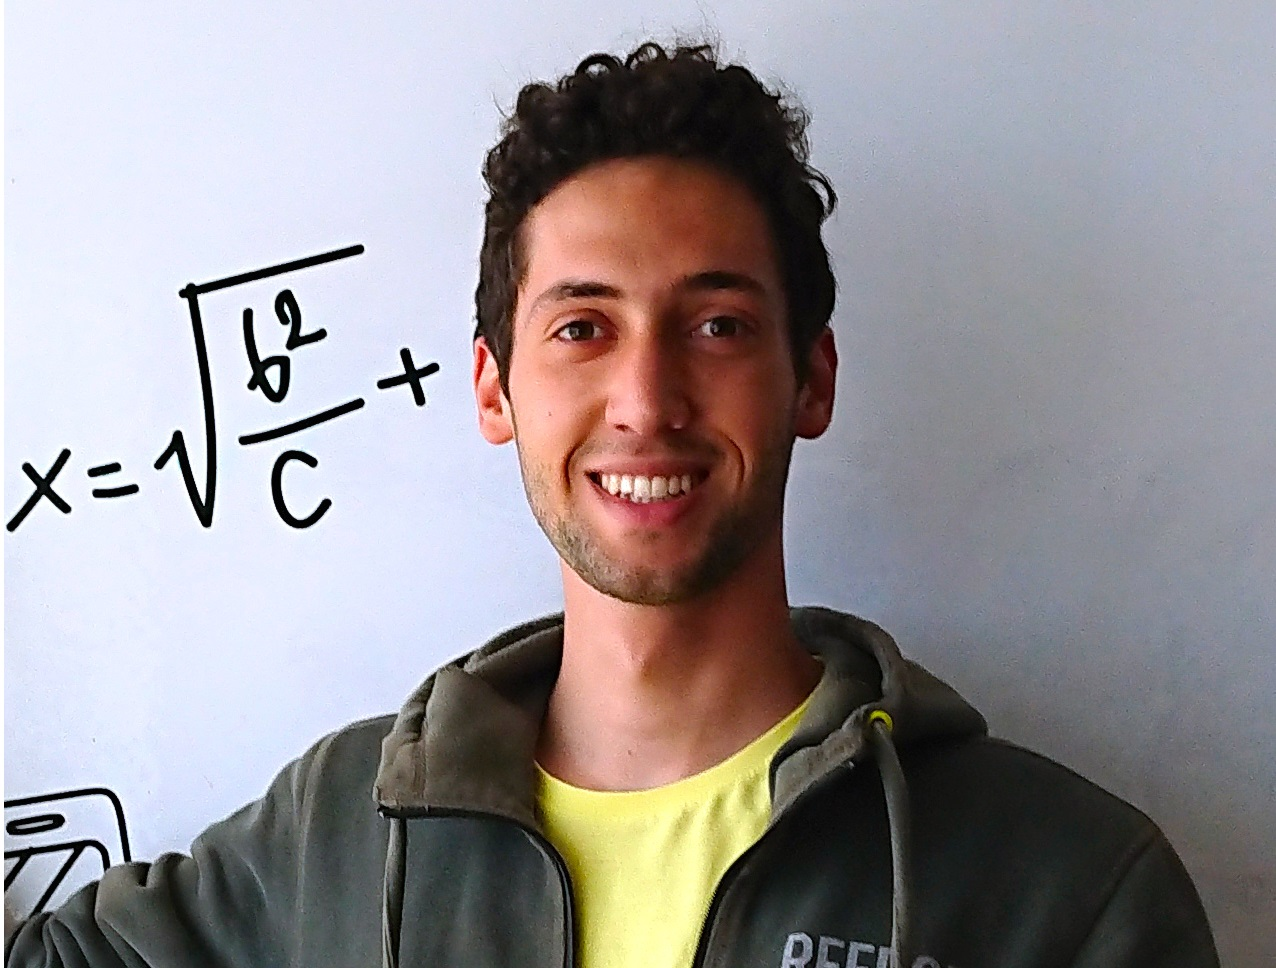
\includegraphics[width=1\textwidth]{photo}
\end{minipage}      
\begin{minipage}{0.7\linewidth}
    \MyName{Igor Lirussi}
    \sepspace
    \noindent
    % info 
    \hfill {\color{headings}Nazionalità:} Italiana | {\color{headings}Nascita:} 25/12/1995 | {\color{headings} Genere:} M | {\color{headings} Stato civile:} Single
    
    \hfill {\color{headings}\faEnvelope} \href{mailto:igor.lirussi@studio.unibo.it}{igor.lirussi@studio.unibo.it}
    | {\color{headings}\faPhone}  0039 3317055048 
    
    \hfill {\color{headings}GitHub/LinkedIn:} igor-lirussi | {\color{headings}Skype:} igor.lirussi
    
    \hfill {\color{headings}\faMapMarker} via VI Maggio 24, 33030, Forgaria nel Friuli (UD), Italy
 
\end{minipage}


%%%%%%%%%%%%%%%%%%%%%%%%%%%%%%%%%%%%%%%%%%%%%%%%%%%%%%%%%%%%%%%%%%%%%%%%%%%%%%%%
\NewPart{Esperienza Lavorativa}{}
\noindent

\href{https://colors.cmpe.boun.edu.tr}{
\shortEntry{RESEARCH ASSISTANT - ROBOTICA COGNITIVA}
{Ott 2021 - Ott 2022}
{Istanbul (TR) Boğaziçi University: Cognitive Learning and Robotics Laboratory}
{
Robot industriale abilitato a raccogliere un oggetto richiesto. \\ Simulazione particellare per fisica in VR.
 \begin{itemize}
    \item Cognitive Robotics
    \item Virtual Reality
 \end{itemize}
} {IMG/bogazici}
}
\sepspace

\href{https://www.kth.se/is/rpl}{
\shortEntry{RESEARCH ASSISTANT - INTERAZIONE ROBOTICA}
{Apr 2020 - Set 2020}
{Stoccolma (SE) KTH Royal Institute of Technology: Robotic Perception and Learning Department}
{
Creazione di un software per l'interazione in linguaggio naturale con un robot umanoide.
 \begin{itemize}
    \item Human Robot Interaction
    \item Dialog Engines
 \end{itemize}
} {IMG/kth}
}
\sepspace

\href{https://welcome.isr.tecnico.ulisboa.pt/}{
\shortEntry{RESEARCH SCHOLAR - COMPUTER VISION}
{Set 2018 - Set 2019 }
{Lisbon (PT) IST Instituto Superior Técnico: I.S.R. Institute for Systems and Robotics - VisLab}
{
Sviluppo di un software per un robot mobile per riconoscere l'ambiente circostante e muoversi al suo interno.
 \begin{itemize}
    \item Object recognition and Dialog Processing for Human Robot Interaction
    \item SLAM and Visual Navigation Systems
 \end{itemize}
} {IMG/ist}
}
%%%%%%%%%%%%%%%%%%%%%%%%%%%%%%%%%%%%%%%%%%%%%%%%%%%%%%%%%%%%%%%%%%%%%%%%%%%%%%%%
\NewPart{EDUCAZIONE}{}
\noindent

\href{https://corsi.unibo.it/2cycle/ComputerScienceEngineering}{
\shortEntry{Magistrale INGEGNERIA E SCIENZE INFORMATICHE}
{Set 2019 - oggi}
{Università di Bologna}
{Distributed Systems, Machine Learning,    Languages, Compilers and Computational Models,    Information Systems,     Concurrent and Distributed Programming,    Programming and Development paradigms,    Web Services and Applications,     Smart City and Mobile Technologies,     Agile, Continuous Integration and Delivery,  } 
{IMG/unibo}
}
\sepspace

\href{https://dsv.su.se/en/}{
\shortEntry{ERASMUS Magistrale}
{Gen 2020 - Lug 2020}
{Università di Stoccolma}
{Decision Making and Business Intelligence, Network Security, Cyber Forensics}
{IMG/stockholmuni}
}
\sepspace

\href{https://ciencias.ulisboa.pt/en}{
\shortEntry{ERASMUS Triennale}
{Set 2018 - Set 2019}
{Università di Lisbona}
{Artificial Intelligence, Operational Research} 
{IMG/ulisboa}
}
\sepspace

\href{https://corsi.unibo.it/1cycle/ComputerScienceEngineering}{
\shortEntry{Triennale INGEGNERIA E SCIENZE INFORMATICHE}
{Set 2014 - Set 2019}
{Università di Bologna}
{Software Engineering, Embedded Systems and IoT, Automatic Controls, Mobile Application Programming, Operating Systems, Object-Oriented Programming, Network Programming, Telecommunications Networks, Law for Information Technology, Fundamentals of Image Processing, Databases, Algorithms and Data Structures, Computer Architecture, C Programming}
{IMG/unibo}
}

%%%%%%%%%%%%%%%%%%%%%%%%%%%%%%%%%%%%%%%%%%%%%%%%%%%%%%%%%%%%%%%%%%%%%%%%%%%%%%%%
\NewPart{ Abilità Tecniche \& Software }{}
\begin{minipage}[t]{0.67\textwidth} 
    \begin{itemize}
    \item Buona padronanza dei linguaggi di programmazione/mark-up di alto e basso livello (HTML-CSS, Assembly, C, C\#, Java, Scala, Python, SQL, Bash scripting).
    \item Conoscenza avanzata degli algoritmi Digital Image Processing/Image Elaboration/Template Matching.
    \item Competenze avanzate in programmi di editing video e foto.
    \item Buona conoscenza del calcolo ad alte prestazioni e data-intensive, Machine Learning e BI.
    \item Discreta padronanza di software per l'automazione, dinamica interna di microcontrollori, sistemi embedded e funzionamento di sensori e attuatori meccanici.
    \end{itemize}
\end{minipage}
%
\begin{minipage}[t]{0.32\textwidth} 
\begin{tabular}[t]{ l l }
\software{IMG/software/git}  & Git/GitHub Actions-Projects\\
\software{IMG/software/opencv}  & OpenCV\\
\software{IMG/software/unity} & Unity \\
\software{IMG/software/latex}  & Latex Writing \\
\software{IMG/software/ros}  & ROS\\
\software{IMG/software/office} & Office Suite
\end{tabular}
\end{minipage}

%%%%%%%%%%%%%%%%%%%%%%%%%%%%%%%%%%%%%%%%%%%%%%%%%%%%%%%%%%%%%%%%%%%%%%%%%%%%%%%%
\NewPart{Lingue e Interessi}{}
\hspace{3mm}
\begin{minipage}[t]{0.33\textwidth} 
%Lingue (ISO 639-1)
\begin{tabular}[t]{ l c l }
\flag{IMG/flag/it} & IT & Madrelingua \\
\flag{IMG/flag/gb} & EN & \href{https://github.com/igor-lirussi/Curriculum-Vitae/raw/main/Certificates/IELTS_LIRUSSI.pdf}{Competenza completa}\\
\flag{IMG/flag/pt} & PT & \href{https://github.com/igor-lirussi/Curriculum-Vitae/raw/main/Certificates/cert_PT_LIRUSSI.pdf}{Livello conversazione}\\
\flag{IMG/flag/sv} & SV & \href{https://github.com/igor-lirussi/Curriculum-Vitae/raw/main/Certificates/cert_SE_LIRUSSI.pdf}{Principiante}\\
%\flag{IMG/flag/tr} & TR & Basic level\\
%\flag{IMG/flag/de} & DE & A2 & \href{https://github.com/igor-lirussi/Curriculum-Vitae/raw/main/Certificates/cert_DE_LIRUSSI.pdf}{Basic level}\\
\end{tabular}
\end{minipage}
%
\begin{minipage}[t]{0.64\textwidth} 
\begin{tabular}[t]{l l}
\href{https://site.unibo.it/startupdayunibo/en/}{Vincitore "Le nuove 30 idee emergenti 2021, StartUp Day - Unibo"}\\
Corso di primo soccorso per aziende teorico e pratico.\\
Appassionato di cucina e sport\\
Donatore di sangue e volontario al Banco Alimentare.\\
\end{tabular}
\end{minipage}


%%% References

\end{document}
